%!TEX TS-program = lualatex
%!TEX encoding = UTF-8 Unicode

% I use LuaLaTex by default so that I get full UTF-8 support, which simplifies
% when using mixed language.

\documentclass[sigconf,anonymous,review]{acmart}
\setcopyright{none}  % suppress copyright generation
\usepackage{lipsum}
\usepackage{xspace}

%% Change this to change the name of the system
\newcommand{\system}[0]{\emph{Kwisatz}\xspace}

\author{Tony Mason}

\title{\system}
\subtitle{Enabling Activity Context}

% These are marks for inserting comments. Feel free to edit as needed!
\newcommand{\nb}[2]{{\yellowbox{#1}\triangles{#2}}}
\newcommand{\nbc}[3]{
 {\colorbox{#3}{\bfseries\sffamily\scriptsize\textcolor{white}{#1}}}
 {\textcolor{#3}{\sf\small$\blacktriangleright$\textit{#2}$\blacktriangleleft$}}}
\newcommand{\version}{\emph{\scriptsize\id}}
\newcommand{\ugh}[1]{#1} % please rephrase
\newcommand{\ins}[1]{#1} % please insert
\newcommand{\del}[1]{} % please delete
\newcommand{\chg}[2]{#2} % please change
\renewcommand{\nb}[2]{\nbc{#1}{#2}{orange}}

% Tony
\definecolor{tmcolor}{rgb}{0.5,0,0.5}
\newcommand\tm[1]{\nbc{TM}{#1}{tmcolor}}

% Margo
\definecolor{miscolor}{rgb}{0.4,0.6,0.2}
\newcommand\MIS[1]{\nbc{MIS}{#1}{miscolor}}

% Ada
\definecolor{adacolor}{rgb}{1.0, 0.5, 0.5}
\newcommand\ada[1]{\nbc{AG}{#1}{adacolor}}

% Sasha
\definecolor{sfcolor}{rgb}{0.2,0.0,0.5}
\newcommand\sasha[1]{\nbc{SF}{#1}{sfcolor}}

\begin{document}


\begin{abstract}
    Our ability to find digital data is reaching a tipping point: brute force
    search techniques are inefficient and searching multiple storage locations
    to find related objects is challenging.  Prior research found using
    contextual clues facilitates finding specific digital objects. Despite
    modern systems collecting vast amounts of contextual information, our
    systems do not provide an efficient mechanism for using that information to
    facilitate more efficient \emph{finding} of digital objects.

    \emph{\system} is our system for collecting, storing, and
    disseminating contextual information we call \emph{activity context} to
    facilitate finding groups of related digital objects regardless of where
    those objects are stored.  We find \emph{\system} is a viable way to
    provide \emph{activity context} and enabling its use by other services and
    applications.
\end{abstract}

\maketitle

\section{Introduction}

\tm{TBD}

\section{Background}

\tm{TBD}

\section{Architecture}\label{sec:Architecture}

\system is logically composed of three major components, each of which is an
essential portion of providing the end-to-end systems level support for
capturing, storing, and utilizing \emph{activity data}.  Each of these
components consists of various smaller components assembled together to provide
the necessary services.

In this section, I lay out the basic architecture of these components.  In
subsequent sections, I will drill down into this architecture and identify key
aspects of the system design. In constructing this architecture, I have
attempted to broadly address what I consider to be the key aspects of these
components, including defining terminology and identifying potential use cases
that may be relevant.  Frequently, I will suggest potential implementations that
would fit within this architecture: there is no expectation that I will
implement even a majority of these potential implementations.  Rather, the goal
of using broad considerations is to assist in ensuring the system architecture
is reasonably flexible. Ultimately, my goal is to demonstrate the architecture
is itself viable as a system service.

\begin{figure}
    \caption{\system Architecture Diagram}\label{fig:architecture}
    \textbf{TODO}
\end{figure}

\begin{description}
    \item[Ingestion] --- the activity data that are presented by various
        services within the system needs to support a rich and robust model in which
        captured data may be converted into a common form that permits
        utilization. \S \ref{sec:Architecture:Ingestion}
    \item[Storage] --- raw activity data, along with extrapolated activity
        meta-data, need to be stored in a format that is scalable and efficient as
        well as supporting a robust utilization model. \S \ref{sec:Architecture:Storage}
    \item[Utilization] --- to realize the benefits of activity data, the system
        must have a useful model for using the activity data. \S \ref{sec:Architecture:Utilization}

\end{description}

\subsection{Ingestion}\label{sec:Architecture:Ingestion}

Activity data can arise from a variety of sources.  For example, because my
primary focus is on utilizing activity data to better inform logical data
organization, I view data storage as being a key source of such information.
Indeed, much of the prior work in this area has focused on utilizing information
about data, including:

\begin{description}
    \item[File Names] --- the \emph{file name} is a time honored way to embed
    information about the file itself.  For example, in
    \emph{Burrito}~\cite{guo2012burrito} the observation is that we capture
    parameter information within the file name.  This is because it is the
    \emph{only} way to safely capture this information in a way that is broadly
    viable across file systems.

    \item[Extended Attributes] --- the \emph{extended attribute} is a mechanism
    that provided a way for applications to create additional meta-data using an
    attribute/key model~\cite{mogul1986representing}.  File systems that support extended attributes maintain
    them as meta-data of the file itself.  Unfortunately, extended attributes
    suffer from two limitations: (1) file systems that do support them provide
    no mechanism for associating files based upon the extended attributes; (2)
    there is no uniform support or implementation of extended attributes.

    \item[File Meta-data] --- most file systems support at least a minimal
    subset of meta-data elements, specifically timestamps and size. There is a
    lack of uniformity of other attributes: POSIX file systems typically support
    ``mode'' bits that represent access permissions as well as potentially other
    behaviors, as well as an access time, modification time, and change time.
    Creation timestamps are often maintained by file systems as well.  A number
    of UNIX-like file systems maintain a creation timestamp.  Windows includes
    the \emph{creation} time of the file and that has been adopted by a number
    of UNIX-derived file systems, including ext4, jfs, and btrfs.  Recent
    changes in Linux include a new system call, \textbf{statx} that permits
    applications to retrieve this information programmatically.

    \item[Directories] --- the traditional hierarchical file system provides a
    mechanism for composing groups of files into a \emph{directory}, which is a
    set of files.  Some file systems restrict a file to being a member of a
    single directory, while others allow a file to be a member of multiple
    directories. The Mutics file system included the ability to create links to
    files.  Modern file systems may implement links as either direct references
    from the directory to the file (``hard links'') or indirect references from
    an entry in the directory to the file (``soft links.'')  They have somewhat
    different semantics.

    \item[Views] --- in semantic file systems~\cite{gifford1991semantic} there
    is less emphasis on reference counted relationships (e.g., hard links) or
    even persistence and more emphasis on creating logical groups (``virtual
    directories'') of files based upon some criteria.

\end{description}

\system does not seek to \emph{replace} any of these existing file storage
mechanisms.  Instead, it focuses on providing rich support for meta-data
\emph{about} digital objects, which includes files but should not be limited
strictly to files.

Meta-data is not strictly limited to the data that is available from the file
system itself.  Further, meta-data may be about digital objects that
\emph{existed} at some point in time but no longer exist: this is a reality of
separating the storage from the meta-data service. Instead of focusing on
maintaining a strongly referenced model, I instead adopt the model of the
Internet, which means that meta-data may reference digital objects that no
longer exist.  Applications that use \system should be aware that the underlying
data could cease to exist and act accordingly.

Other potential sources of meta-data are quite broad and include:

\begin{description}
    \item[Semantic transducers] --- the term \emph{transducer} was first
    introduced as part of semantic file systems~\cite{gifford1991semantic}.  The
    basic idea was that active components would \emph{extract} semantic
    information from the contents of a file and then use it for indexing.
    Indeed, modern indexers work on this basic principle, without making any
    changes to the file system.

    \item[Content classifiers] --- one common use for machine learning is to
    identify the content of specific files, such as images or videos, to
    determine if the given file contains specific content: a cat, for example.
    Such classifiers can be more targeted, such as finding pictures of a
    specific person, or containing a \emph{particular} cat.  This information
    can then be used to cluster files together, such as the ``video reels'' that
    some service providers now give us on our personal devices.

    \item[Hashing] --- a \emph{hash} can be computed on a given file to
    determine if the contents of said file has changed.  For example, this can
    be used by ``cloud storage'' providers to determine if a given file has
    already been uploaded.  Hashing can also be used to determine when files
    have changed.

    \item[Metrics] --- one common approach to information is to establish the
    logical proximity of the files, whether based upon the \emph{content} of the
    file, or the \emph{meta-data} of the file.  For example, plagiarism tools
    like MOSS look for structural similarity (versus simpler textual similarity)
    by comparing the abstract syntax trees of code.  This generates a measure of
    similarity.  The \emph{value} of the metric is not material to this project,
    but the \emph{use} of metrics is because it allows us to create a logical
    distance between the objects.  This can, in turn, be used to \emph{cluster}
    objects that are ``close to'' each other.

    \item[Environment] --- our devices maintain multiple sources of
    environmental information.  For example, location information (\emph{GIS})
    identifies where a device is located at a given time.  Increasingly, our
    devices track other aspects of the environment, including the ambient
    temperature, our vital measurements such as heart rate and blood pressure,
    and even more detailed health information including data from pace makers,
    insulin pumps, and menstrual cycle trackers.  The data from these is likely
    useful in creating associations between extrinsic events and human storage
    usage.

    \item[Social] --- our devices routinely track our social activity: with whom
    we are interacting via text, chat, e-mail, and video call, for example.
    Frequently, as part of this we share information --- information that is
    subsequently stored, modified, and re-shared onwards.  This type of activity
    data can be used to help us identify where information came from, what other
    digital objects were accessed as a result, and establishing data
    relationships based upon usage patterns.  Web sites visited, Reddit posts
    liked, Discord messages exchanged, music listened to, purchases made, and
    even games played can all be used to construct associative relationships
    that make sense to human users.

\end{description}

In general, activity data can be \emph{intrinsic} to the digital object, such as
information based upon its semantic content, it's length, and contents as well
as \emph{extrinsic} to the digital object, such as what applications were used
to access it, where things were done, with whom, etc. The \system architecture
is influenced by my desire to ensure support for a broad range of activity data
sources.

In \S \ref{sec:ingestion} I delve into greater detail about handling activity
data.

\subsection{Storage}\label{sec:Architecture:Storage}

The choice of storage models, while important, is unlikely to give rise to
significant research questions at this juncture: as we begin to understand the
nature of the activity data we anticipate collecting, it is distinctly possible
that new challenges will emerge.  However, we have an extensive body of
knowledge on how to handle high data rates (``drinking from the fire hose'') as
well as scaling approaches for managing potentially large bodies of data.

Thus, while the architecture is fairly neutral with respect to the details here,
I anticipate the initial implementation of this will utilize ``reasonable''
limitations on activity data sources (e.g., curation to avoid excessive data
loads).

An important aspect of the architecture is to propose a model for the data
format that I propose using.  This data format must be able to:

\begin{itemize}
    \item Identify the \emph{source} of the activity data.  This permits
    interpretation of the captured data by any transducer familiar with the data
    generated by the given source.

    \item Specify the \emph{version} of the activity data.  My own review of
    numerous data sources suggests that it is common for many of them to change
    the format of the data over time; typically this \emph{extends} the data
    format (common for systems-related activity data sources, for example) but
    sometimes it involves significant restructuring of the data that is
    available (common for web-based activity data sources.)  By including a
    version, a transducer can determine if it understand the format of this data
    and permits evolution.

    \item Provide an ordering of the activity data.  Typically this would be
    a ``timestamp,'' though there is no reason this needs to be a timestamp
    relative to any other data source.  Further, when there are multiple
    providers of information, the interpretation of this Lamport clock is
    ultimately determined by the transducer. This \emph{allows} both system
    relative and universal clocks but does not dictate their presence nor
    disallow clocks that are shared between activity data providers.

    \item A list of \emph{attributes}.  These are in the format of ``extended
    attributes,'' with both an identifier as well as a value.  This permits
    attributes that can be the same across sources, as well as allow the same
    ``attribute'' to have different meanings for different sources.  This is
    neither required nor prohibited within the \system architecture.  This
    ability provides very broad support for activity data, as well as \emph{post
    hoc} supplementation by transducers.

    \item The \emph{raw data} originally captured by the activity data provider.
    This allows the capture of information without requiring interpretation at
    the time it is captured. In cases where there is no additional raw data,
    this can remain empty.  Note that this is \emph{not} anticipated as being an
    area in which to store the digital object's data.

\end{itemize}

As a concrete example, I have implemented an activity data provider that scans
and captures the change data from the NTFS USN Journal on a Windows 11 computer.
The raw data is captured, and then certain elements of the data can be
augmented.  For instance, the raw data provides a \emph{file id} that is used to
obtain the name of the file.  Similarly, the raw data also provides a
\emph{directory id} that is used to obtain the path of the containing directory.
This is relative to the NTFS volume (which does \emph{not} include a drive
letter.)  Thus, the transducer for this can utilize the \emph{volume id} to map
to the current drive letter, making this name available for ordinary Windows
applications (which tend to use drive letters, even though they aren't visible
to the NTFS file system controlling a given volume.)

Subsequent to this, I envision a separate transducer that can be used to compute
the hash value of the file's contents.  That hash value could then be
incorporated into the attributes list of the corresponding change journal record
(assuming the file has not changed by the time the hash value has been computed,
of course.)

This data format can then be easily captured as a JSON expression, which can
then be used to store the relevant data in a database (e.g., DynamoDB or
MongoDB, for example.)  This decouples the specific details of how the data is
stored from the format required of the data gathering elements.

I discuss this in greater detail in \S \ref{sec:storage}.

\subsection{Utilization}
\label{sec:Architecture:Utilization}

It is essential to have a model for utilizing activity data in order to realize
its potential.  The \system architecture is generalized with an eye towards
permitting a range of potential use cases.

Underlying the structure of the data are elements that I anticipate will be used
to establish relationships.  For example, the \emph{metric} concept described
earlier (\S \ref{sec:Architecture:Ingestion}) naturally fits with data
clustering mechanisms.  This is consistent with a \emph{graph} representation in
which the edges correspond to some relationship and the weight of the edge
corresponds to a metric. Similarly, it can be useful to add labels to the data,
in order to understand specific characteristics of that information.  The
emphasis on using graph modeled storage (\S \ref{sec:Architecture:Storage}) is
also consistent with this.  Thus, the logical way to utilize this information is
to focus on exploiting the inherent graph structure of the data.

Given this model of exploring graph data, it makes sense to then consider using
an existing graph query language --- reserving the right to limit its use to
some subset as part of the exploratory work I am doing.  One motivation for this
would be that such languages \emph{already} work with commonly used graph
databases and thus leverage prior work in using graph structured information
effectively.

I discuss this in greater detail in \S \ref{sec:utilization}.

\section{Ingestion}
\label{sec:ingestion}

There is no single mechanism for retrieving activity data because each source
for such data provides it in multiple different ways.  Thus, for the purposes of
our analysis we found it useful to categorize data sources based upon how we
retrieved the information.  Thus, one of the jobs of an ingestion agent is to
retrieve the data and then put it into our common format, which will permit us
to use that information for subsequent processing and analysis.

\subsection{Models}\label{sec:ingestion:models}

In our work we have found multiple ways that activity data can be retrieved:

\begin{description}
    \item[Systems API] --- one common approach for retrieving activity data is
    via an operating system defined application programming interface (API).
    For example, the eBPF mechanism commonly found in several operating systems
    represents a general mechanism for retrieving activity data from a variety
    of sources.  To that extent it provides a general extensible framework for
    activity data, with the format of the data being returned dependent upon its
    source.  Similarly Microsoft Windows has an operating system mechanism known
    as \emph{Event Tracing for Windows} that is used extensively by Microsoft to
    provide detailed activity data for essentially all portions of their
    operating system.  A more focused interface on Windows is the USN Journal,
    which is supported by the NTFS file system.  Each of these provides a
    specific interface for retrieving data that is directly visible to the local
    system.

    \item[Web APIs] --- another common approach is to provide web interfaces to
    service providers that can be used to retrieve information, including
    activity data.  Such web APIs may be directly accessible on the local system
    or may involve contacting a remote service provider.  In each of these cases
    an agent can capture this data and store the relevant activity data in our
    common database. The specific details of the web API vary by provider.
    For example, the Dropbox service on a local system supports querying for changes via a
    web API against the local system.  The Github API includes the ability to
    query for events on a polling basis.

    \item[Web hooks] --- some web services do not provide a direct event query
    interface and instead require creation of an intermediate agent via a
    registered web hook.  In such a case, the web service provider is given the
    address of a distinct publicly available web service which is invoked
    periodically with event information. Because the web hook must be publicly
    available an agent collecting data from such a service requires both a local
    agent on the machine where the activity data is being recorded as well as a
    public agent on an internet facing public machine.

    \item[Manual Scanning] --- some services do not provide any simple mechanism
    for detecting activity data directly.  In such a case it is possible to
    construct an activity agent that manually scans for changes.  One example if
    this would be the \emph{rclone} facility which uses brute force scanning of
    a storage location to determine ``what has changed'' and then uses that
    information to synchronize copies of that data on a secondary copy.  While
    simple, this approach is well-known and can be used when building a activity
    data gathering agent.
\end{description}

These various techniques are all \emph{possible} but have potentially radically
different performance characteristics that may limit their utility.  Thus, we
wanted to construct at least one example of each in order to better understand
the viability of using activity data collection agents for each of these classes
of service.

In some cases we found it was possible to create indirect monitoring mechanisms.
For example, one service we commonly use --- \emph{Overleaf} --- does not have a
web monitoring API.  However, it \emph{does} integrate with Github repositories
and thus we can simulate tracking Overleaf change data by using the Github APIs.

Another approach, which we did not explore for this work, would be to use API
aggregation services such as \href{https://zappier.com}{Zappier}.  Such
aggregation sites combine web APIs and may be a fruitful way to extract
additional activity data from a broad range of sources.

We chose a single example of each of these types of activity data retrieval.
This allows us to explore the space broadly and gain further insight into the
viability of using such sources.

\begin{figure}
    \centering
    \caption{Google Drive API Web Hook}\label{fig:google-web-hook}
    \begin{tabular}{c}
        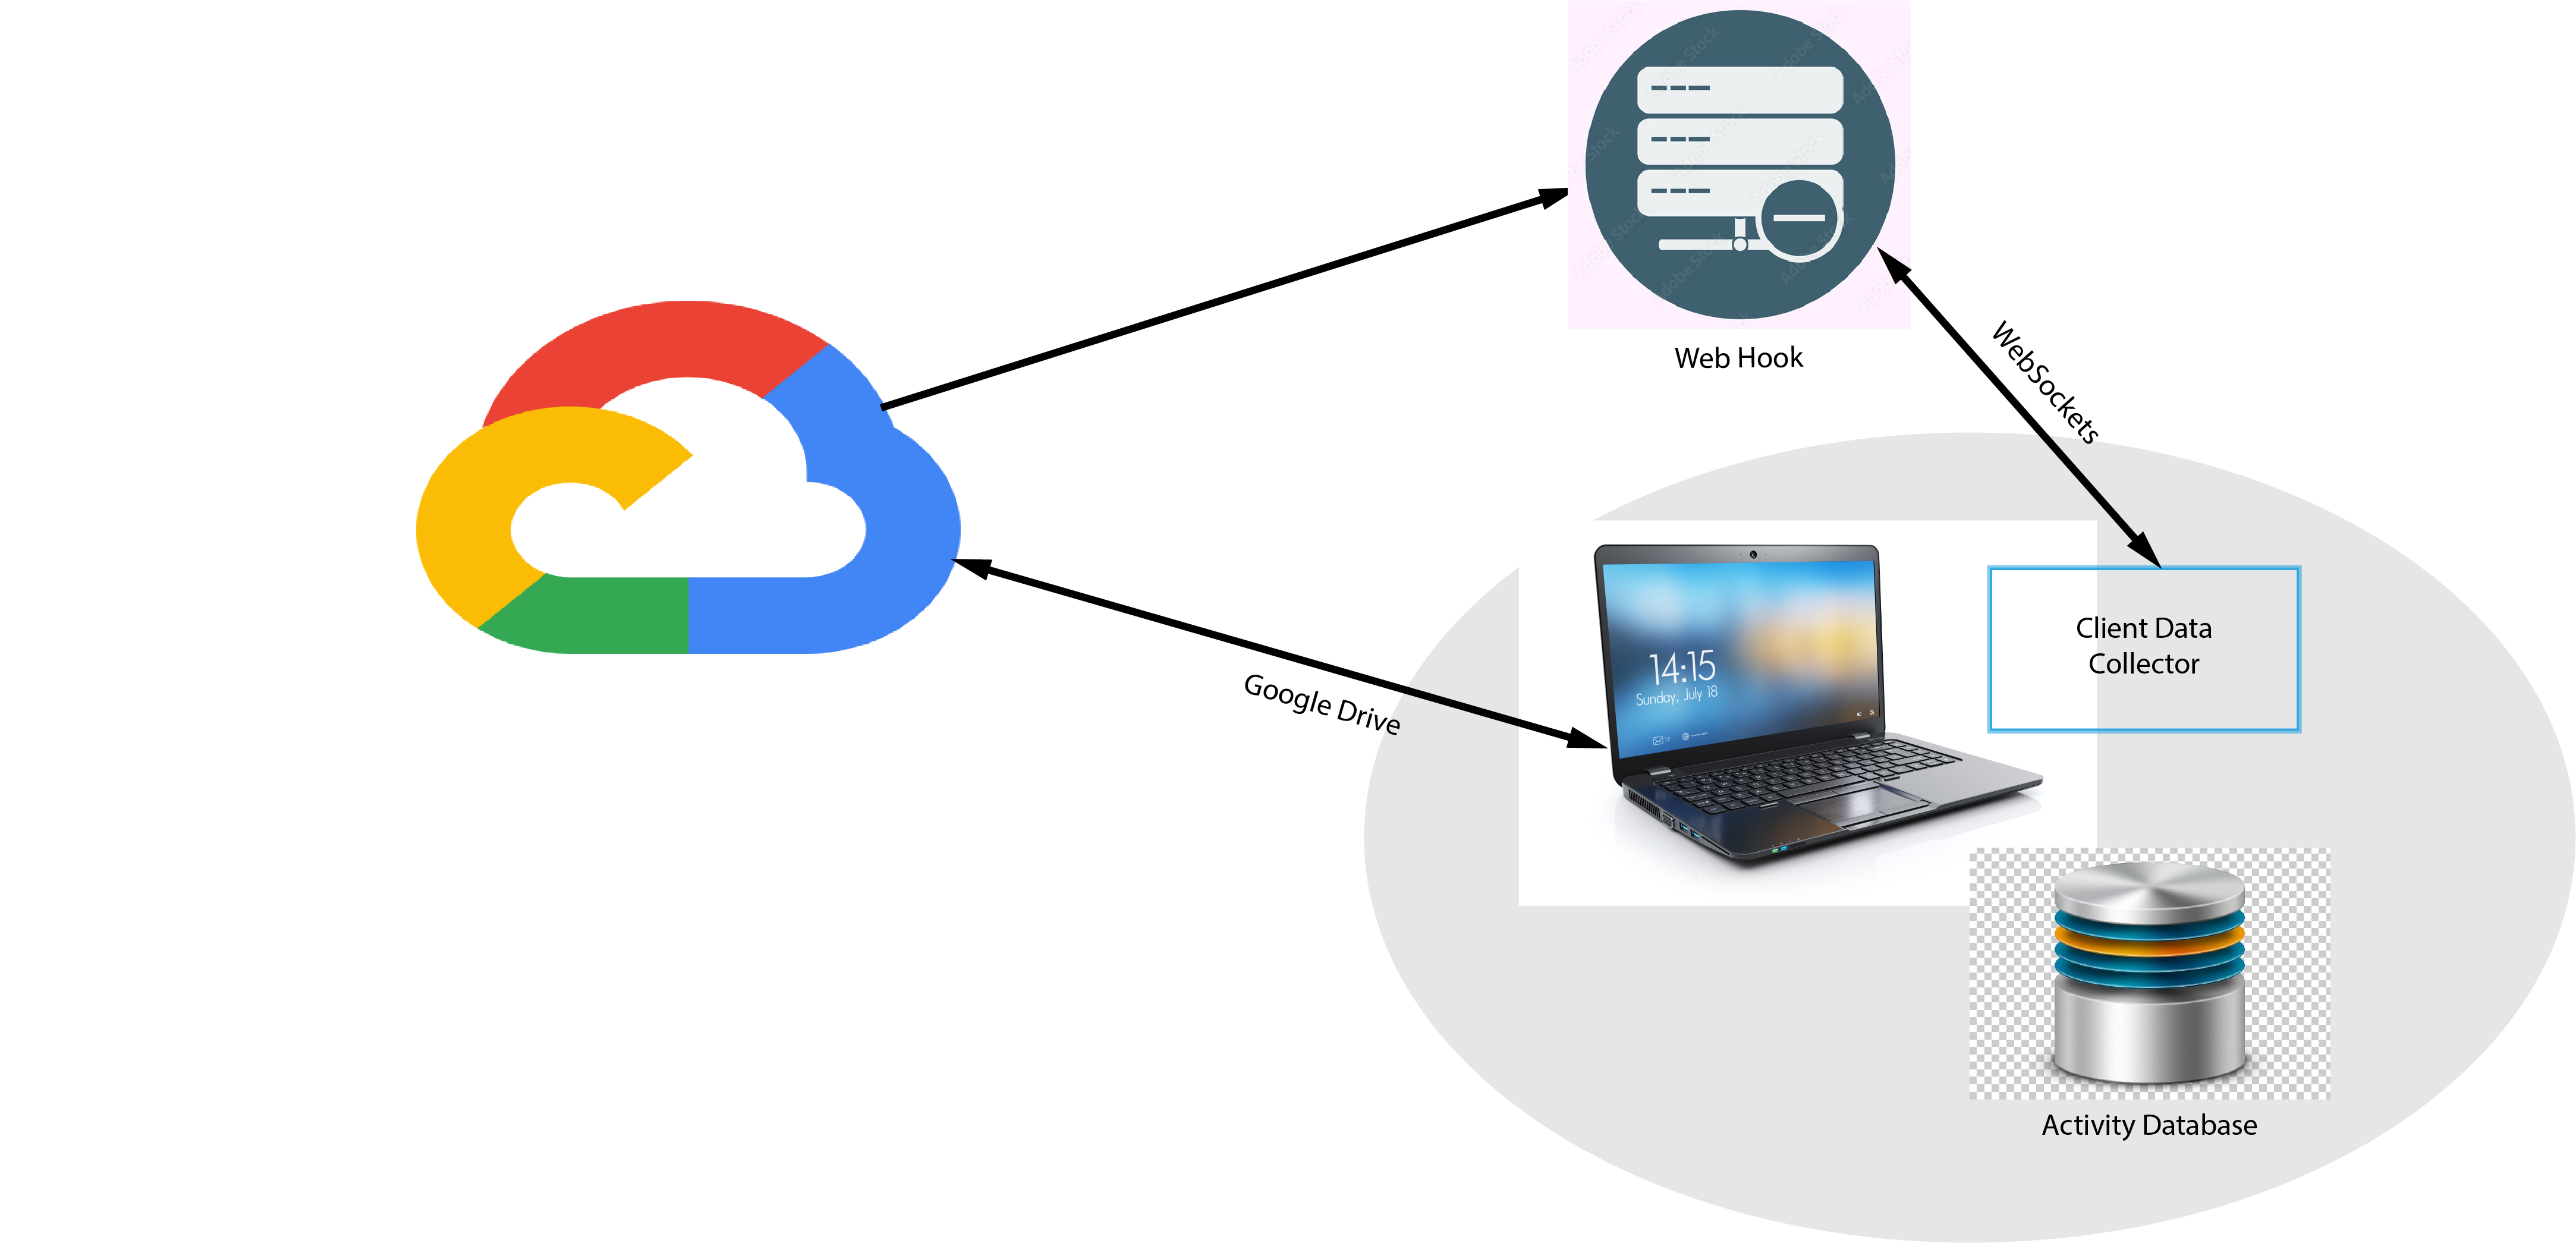
\includegraphics[width=0.45\textwidth]{figures/google-cloud-monitor.png}
    \end{tabular}
\end{figure}

\begin{itemize}
    \item For our systems API example we chose to use the Update Sequence Number
    (USN) Journal support provided by the NTFS File system in
    Windows~\cite{huang2012research}.  This system provides a curated view of
    file system activity on drives where the USN journal has been enabled. By
    default the USN journal is enabled on the system drive and may be optionally
    enabled on other drives.  This is a publicly documented API, has good
    performance, and provides a curated level of information that provides
    benefit without being ``too broad.''
    \item For our Web API example we use the Dropbox cloud storage
    system.  This relies upon a local service on a specific computer.  This
    service can be used to monitor activity on the Dropbox system.  We used a
    standard Dropbox installation on Windows, Version 154.4.5353. \tm{Add
    citation for Dropbox?}
    \item For our Web Hook example we use the Google Drive API.  To do this we
    constructed a public facing web service that we could
    register with Google to receive changes (the ``web hook'').  We also
    constructed a local service that could run on a desktop computer to obtain
    the necessary credentials and provide them to Google as well as gather up
    data from our public facing web service.  We show a simple diagram of this
    arrangement in Figure \ref{fig:google-web-hook}. Our implementation was
    simple and relied upon pre-installed certificates between client and webhook
    to provide cross-system authentication.
    \item For our manual scanning example, we chose to use \tm{TBD}.

\end{itemize}

While building the various activity data collection agents we made a number of
observations around potential challenges to constructing such agents:

\begin{itemize}
    \item It is broadly useful to have \emph{curation} over the data source.
    One of the challenges of reading from a ``fire hose'' is that the
    ``signal-to-noise'' ratio can be low.  Instead, the emphasis should be on
    capturing discrete events that are useful.

    \item To use labels to identify the specifics of particular relationships
    and properties to capture information that can be used later requires a
    level of understanding of what the data source provides and how that
    compares with other data sources.  For example, timestamps might be
    collected using a different interpretation of time zero so to use this
    information requires some means of comparing such cross-domain values.
    Similarly, in a system where multiple objects are grouped together via the
    naming system (e.g., files within a directory) it is useful to capture that
    relationship when the activity agent is recording information.

    \item \tm{TBD}
\end{itemize}

\subsection{Evaluation}

Our evaluation of these activity data collection agents involves considering
several key factors:

\begin{itemize}
    \item The time and complexity of the code needed to implement the agent.
    \item The amount of data the agent generates per unit time.
    \item The performance impact of the agents on the system.
    \item \tm{TBD}
\end{itemize}

\tm{So, the point here is to provide a straight-forward framework for evaluating
the overhead associated with these activities as part of the evaluation.}

\section{Storage}
\label{sec:storage}

A ``labeled property graph'' includes:

\begin{description}
    \item[node] --- in traditional mathematical graph descriptions this is the
    \emph{vertex}.  For my work this corresponds to a digital object, such as a
    file in a file system, a value in a key/value store, etc. Nodes within my/
    system have \emph{structure} because it must codify ``where'' the actual
    digital object is located in addition to the other information needed.  For
    practical purposes I think of the ``location'' as being a uniform resource
    identifier (\href{https://datatracker.ietf.org/doc/html/rfc8820}{URI}.)  The
    benefit of this paradigm is that it relies upon an existing standard for
    identifying objects, which is sufficient for my work.

    \item[relationship] --- in traditional mathematical graph descriptions this
    is the \emph{edge} that connects a pair of vertices.

    \item[identifier] --- this identifies the graph element (node or relationship).

    \item[label] --- this is a descriptive property related to the node or
    relationship.  For example, a label might identify that a node is a
    \emph{file} versus a \emph{value} in a key/value store.  Similarly, a label
    associated with a relationship would establish \emph{what} type of
    relationship this represents, such as a \emph{derived from} or a
    \emph{contained by} relationship.

    \item[property] --- this is essentially a key/value pair, where the key
    represents the property and the value represents the data associated with
    that property.  My goal is to permit some structure to a property, so that
    it may have a version associated with it, permitting more flexible upgrades
    to the format of the data.

\end{description}

I choose this model because it fits the data we collect and permits exploration
of augmenting the model with distinct agents capable of adding specific property
information as well as relationships.

Thus, \emph{nodes} in this model represent data objects and activity events.
This can be used to create different types of relationships.  For example,
\emph{causal} relationships would show a flow from one data object to a second
data object based upon an activity event that ``explains'' that transformation.
This would be a way to capture \emph{provenance} information.  However, the
model is not limited to this type of relationship.  For example, data objects
created when the same web page was being accessed could be identified by using
an activity event node representing the web page access.  This sort of
contextual relationship is useful for finding related data objects that are not
causally linked.  This might occur, for example, when writing code.  A developer
could be shown other files they created when looking at the same page, allowing
them to find that prior work.

Because our goal is to find assocations via explicit and inferred contextual
information, we describe activity \emph{events} and \emph{contexts}.  An
activity \emph{event} is a node that an activity provider inserts to represent
some specific information about \emph{what} happened.  An activity
\emph{context} is created on demand and associates a set of activity events with
another object (e.g., a data object).  For a data object, this creates a
relationship between the object and potentially related activity events.

Thus, the expectation is that we can retrieve the most recent instance of an
activity event of interest (where I leave defining \emph{of interest} to be
determined.)  For a simple demonstration, it likely makes sense to simply have a
list of the ``most recently added'' instance for each activity provider and
simply form the activity context by associating it.  As the number of activity
providers increases, further work will likely be needed to enable scaling.

Thus, an \emph{activity context} can be associated with other objects.  This
will permit us to subsequently examine the context of operations that were
ongoing at the time of interesting events.

This leads to a number of interesting questions to explore:

\begin{itemize}
    \item Does it make sense to maintain temporal relationships in this fashion;
    in other words, does the newest activity context point back to the previous
    activity context, or do the activity events point back to the older activity
    event?

    \item Should an activity context be something added implicitly (e.g., each
    time one creates a \emph{data} node, should the system automatically
    associate an activity context with it,) or explicitly (e.g., only when
    performed by an external agent.)

    \item How do we garbage collect this information?  That's not likely an
    important question to answer for prototypes, but it will become an important
    question as systems such as this emerge.

\end{itemize}

\subsection{Use Cases}

While we expect numerous potential uses of activity context to be found, we have
identified three interesting cases that we have used to drive our own
exploration of activity context.

\begin{description}
    \item[Search] --- search services are ubiquitous in storage
    solutions.  Prior work has clearly identified that activity context
    information can be used to improve search
    outcomes~\cite{vianna2019searching}.  Further, the ability to search across
    distinct storage domains provides benefits to users over the iterative
    search mechanisms they typically use.
    \item[Data Browser] --- our group did preliminary experimentation with an
    alternative file browser that worked using associations, rather than
    limiting themselves to hierarchical structure.  This is also reminiscent of
    work done in the Human-Computer Interface (HCI) community regarding
    collaborative non-hierarchical data organization
    tools~\cite{collins2007tabletop}.  Our richer contextual environment is one
    that supports further exploration of alternative data visualization techniques.
    \item[TBD] --- \tm{Need to find some other good use case here.}
\end{description}

\subsection{Evaluation}

We evaluate the resource consumption requirements of our storage of this data.
To do so we consider:

\begin{itemize}
    \item The rate at which activity data is added to the database, including
    any additional overhead associated with our databases.
    \item The processor utilization for storing this data.
    \item \tm{TBD}
\end{itemize}


\section{Utilization}
\label{sec:utilization}

While prior work~\cite{vianna2019searching} has established benefits of using
activity context for improving search, we have restricted our initial
implementation to capturing a subset of the data suggested by previous work.
Thus, we need to demonstrate that even this subset provides general utility.

\subsection{Use Cases}

\subsection{Evaluation}

\section{Conclusion}

\tm{The idea that using behavioral advertising information could be beneficial
to file search would potentially be of interest to aggregation companies
because it would encourage use of these tools willingly: a ``free'' service
subsidized by advertising.}


\nocite{*}
\clearpage

\bibliographystyle{ACM-Reference-Format}
\bibliography{bib/indaleko.bib}

\end{document}

